% !TeX program = xelatex
\documentclass[a4paper,10pt]{article}

% ============================================================================
% សន្លឹកកិច្ចការសិស្ស ស-ខ្មៅ (Student Guided-Inquiry Worksheet - Grade 8 ALG51)
% បរិបទ៖ ថ្នាក់រៀនគ្មានស្លាយ LCD – ១.១-១.៣ សញ្ញាណឯកធា ឯកធាដូចគ្នា និងដឺក្រេនៃឯកធា (២ ទំព័រ A4)
% ============================================================================
\usepackage[a4paper, left=0.90cm, right=0.90cm, top=0.75cm, bottom=0.85cm, footskip=0.45cm]{geometry}
\usepackage{amsmath, amssymb}
\usepackage{unicode-math}
\usepackage{fontspec}
\usepackage{array, colortbl}
\usepackage[table]{xcolor}
\usepackage{enumitem}
\usepackage{pifont}
\usepackage{fancyhdr}
\usepackage{lastpage}
\usepackage{tikz}
\usepackage[most]{tcolorbox}
\usetikzlibrary{calc, arrows.meta, positioning, babel}

\makeatletter
\let\@expl@@@mark@update@singlecol@structures@@\relax
\makeatother

\providecommand{\NGSFindFonts}{%
  \IfFileExists{C:/Windows/Fonts/cambria.ttc}{%
    \def\NGSSysPath{C:/Windows/Fonts/}%
    \def\NGSUserPath{C:/Users/KIT/AppData/Local/Microsoft/Windows/Fonts/}%
  }{%
    \IfFileExists{./fonts/KhmerOSsiemreap.ttf}{\def\NGSSysPath{./fonts/}\def\NGSUserPath{./fonts/}}{%
    \IfFileExists{../fonts/KhmerOSsiemreap.ttf}{\def\NGSSysPath{../fonts/}\def\NGSUserPath{../fonts/}}{%
    \IfFileExists{../../fonts/KhmerOSsiemreap.ttf}{\def\NGSSysPath{../../fonts/}\def\NGSUserPath{../../fonts/}}{%
    \IfFileExists{../../../fonts/KhmerOSsiemreap.ttf}{\def\NGSSysPath{../../../fonts/}\def\NGSUserPath{../../../fonts/}}{%
    \IfFileExists{../../../../fonts/KhmerOSsiemreap.ttf}{\def\NGSSysPath{../../../../fonts/}\def\NGSUserPath{../../../../fonts/}}{%
    \IfFileExists{../../../../../fonts/KhmerOSsiemreap.ttf}{\def\NGSSysPath{../../../../../fonts/}\def\NGSUserPath{../../../../../fonts/}}{%
    \IfFileExists{../../../../../../fonts/KhmerOSsiemreap.ttf}{\def\NGSSysPath{../../../../../../fonts/}\def\NGSUserPath{../../../../../../fonts/}}{%
      \def\NGSSysPath{../../../../../../../fonts/}\def\NGSUserPath{../../../../../../../fonts/}%
    }}}}}}}%
  }%
}
\NGSFindFonts

\setmathfont[Path={\NGSSysPath}, FontIndex=1, Scale=1.02]{cambria.ttc}
\defaultfontfeatures{Ligatures=TeX}

\setmainfont[
  Path={\NGSUserPath},
  Extension=.ttf,
  Script=Khmer,
  BoldFont={KhmerOSsiemreap},
  BoldFeatures={FakeBold=1.8},
  ItalicFont={KhmerOSsiemreap},
  ItalicFeatures={FakeSlant=0.25},
  BoldItalicFont={KhmerOSsiemreap},
  BoldItalicFeatures={FakeBold=1.8, FakeSlant=0.25}
]{KhmerOSsiemreap}

\newfontfamily\muol[Path={\NGSUserPath}, Extension=.ttf, Script=Khmer]{KhmerOSmuollight}
\newfontfamily\TimesEn[Path={\NGSSysPath}, Extension=.ttf, BoldFont={timesbd}, ItalicFont={timesi}, BoldItalicFont={timesbi}]{times}

\XeTeXlinebreaklocale "km"
\XeTeXlinebreakskip = 0pt plus 1pt minus 0.1pt

\definecolor{panelgray}{gray}{0.94}
\definecolor{headgray}{gray}{0.86}

\pagestyle{fancy}
\fancyhf{}
\renewcommand{\headrulewidth}{0pt}
\fancyfoot[L]{\fontsize{8pt}{10pt}\selectfont អនុវិទ្យាល័យព្រះក្រសាំង \en{|} គណិតវិទ្យា ថ្នាក់ទី៨ \en{|} មេរៀនទី៥ (១.១--១.៣ សញ្ញាណឯកធា ឯកធាដូចគ្នា និងដឺក្រេ)}
\fancyfoot[R]{\fontsize{8.2pt}{10pt}\selectfont ទំព័រ \en{\thepage\ / \pageref{LastPage}}}

\setlength{\parindent}{0pt}
\setlength{\parskip}{0pt}
\setlength{\tabcolsep}{4pt}

\newcommand{\en}[1]{{\TimesEn #1}}
\newcommand{\enbf}[1]{{\TimesEn\textbf{#1}}}
\newcommand{\unit}[1]{\,\text{\en{#1}}}
\newcommand{\cnum}[1]{{\fontsize{10pt}{12pt}\selectfont\ding{\numexpr171+#1\relax}}}
\newcommand{\chk}{\tikz[baseline=-0.15ex]\draw[black, line width=0.8pt] (0,0) rectangle (0.25cm,0.25cm);}
\newcommand{\dotline}[1]{\makebox[#1]{\dotfill}}

\newcolumntype{L}[1]{>{\raggedright\arraybackslash}p{#1}}
\newcolumntype{C}[1]{>{\centering\arraybackslash}p{#1}}

\newcommand{\secbar}[2]{%
  \vspace{3pt}
  \noindent\colorbox{headgray}{\parbox{\dimexpr\linewidth-2\fboxsep\relax}{%
    \vspace{1.5pt}{\muol\fontsize{9.5pt}{13.5pt}\selectfont #1}\hfill{\fontsize{8.5pt}{12pt}\selectfont\textbf{#2}}\vspace{1.5pt}%
  }}\par\vspace{3pt}
}

\begin{document}
\fontsize{9.5pt}{14.2pt}\selectfont

% ============================================================================
% ទំព័រទី១៖ ក្បាលសន្លឹកកិច្ចការ + E1 + E2 + E3
% ============================================================================
\begin{tcolorbox}[enhanced, sharp corners, colback=white, colframe=black, boxrule=1.0pt, top=4pt, bottom=4pt, left=6pt, right=6pt]
  \begin{center}
    {\muol\fontsize{10.5pt}{15pt}\selectfont សន្លឹកកិច្ចការសិស្ស — មេរៀនទី៥៖ កន្សោមពីជគណិត \enbf{(}១.១--១.៣ ឯកធា\enbf{)}}\\[2pt]
    {\footnotesize សៀវភៅសិក្សាគោលថ្នាក់ទី៨ ទំព័រ ៥១--៥៣ \en{|} រុករកដោយតារាង \en{Frayer} និងអត្តសញ្ញាណអថេរ (គ្មានស្លាយ \en{LCD})}
  \end{center}
  \vspace{2pt}
  \hrule height 0.5pt
  \vspace{4pt}
  ឈ្មោះសិស្ស៖ \dotline{5.3cm} ថ្នាក់៖ \dotline{2.0cm} ដៃគូទី៖ \dotline{2.0cm} កាលបរិច្ឆេទ៖ \dotline{3.3cm}
\end{tcolorbox}

% -------------------- ផ្នែកទី១៖ E1 ENGAGE --------------------
\secbar{ផ្នែកទី១ ៖ បេសកកម្មភ្ជាប់បញ្ហា \enbf{(E1 — Engage)} — គូបទ្រនុង $2a$ និងអាថ៌កំបាំងដឺក្រេ}{\en{3} នាទី (ទស្សន៍ទាយមុនរៀន)}

\begin{tcolorbox}[enhanced, sharp corners, colback=panelgray, colframe=black, boxrule=0.8pt, top=3pt, bottom=3pt, left=6pt, right=6pt]
  \begin{minipage}[c]{13.4cm}
    ១) គូបមួយមានទ្រនុងប្រវែង $2a$ (សៀវភៅគោល ទំ.៥១) ៖ ផ្ទៃក្រឡាមុខខាងនីមួយៗស្មើ $(2a)^2 = \dotline{1.4cm}$ និងមាឌគូបស្មើ $(2a)^3 = \dotline{1.4cm}$ ។\\[2pt]
    ២) \textbf{បេសកកម្មទស្សន៍ទាយ៖} តើឯកធាច្រើនអថេរ $x^2yb^3$ មានដឺក្រេស្មើប៉ុន្មាន?\\[1.5pt]
    \hspace*{0.4cm}\chk\ មតិទី១៖ ដឺក្រេស្មើ $3$ (យកនិទស្សន្តធំជាងគេ) \quad
    \chk\ មតិទី២៖ ដឺក្រេស្មើ $5$ ($2+3$) \quad
    \chk\ មតិទី៣៖ ដឺក្រេស្មើ $6$ ($2+1+3$)
  \end{minipage}\hfill
  \begin{minipage}[c]{4.8cm}
    \centering
    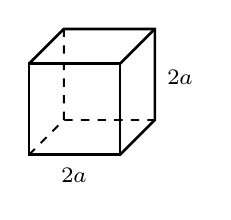
\begin{tikzpicture}[scale=0.68, every node/.style={font=\footnotesize, text=black}]
      \draw[black, line width=0.95pt] (0,0) rectangle (1.7,1.7);
      \draw[black, line width=0.95pt] (1.7,0) -- (2.35,0.65) -- (2.35,2.35) -- (0.65,2.35) -- (0,1.7);
      \draw[black, line width=0.95pt] (1.7,1.7) -- (2.35,2.35);
      \draw[black, line width=0.7pt, dashed] (0,0)--(0.65,0.65)--(2.35,0.65) (0.65,0.65)--(0.65,2.35);
      \node[below=1pt] at (0.85,0) {$2a$};
      \node[right=1pt] at (2.35,1.45) {$2a$};
    \end{tikzpicture}
  \end{minipage}
\end{tcolorbox}

% -------------------- ផ្នែកទី២៖ E2 EXPLORE --------------------
\secbar{ផ្នែកទី២ ៖ រុករកសញ្ញាណឯកធា ឯកធាដូចគ្នា និងដឺក្រេ \enbf{(E2 — Explore)}}{\en{11} នាទី (ពិភាក្សាដៃគូ)}

\textbf{ក. សកម្មភាពទី១ (តារាងញែកកន្សោមតាមលក្ខខណ្ឌប្រមាណវិធី)៖} គេឱ្យកន្សោមពីជគណិតចំនួន ៨ ៖
\[ \frac{1}{5}x^2y \quad;\quad 3x^2 + 2 \quad;\quad 25 \quad;\quad -\frac{2}{3}a^4bc^2 \quad;\quad \frac{a}{x^2} \quad;\quad 2\sqrt{3}yt^2 \quad;\quad zx^2a^3b^4 \quad;\quad 5\sqrt{x} \]
ចូរពិភាក្សាជាដៃគូ រួចបែងចែកកន្សោមទាំង ៨ ចូលក្នុងតារាងខាងក្រោម៖

\vspace{2pt}
{\renewcommand{\arraystretch}{1.38}
\begin{tabular}{|L{9.1cm}|L{9.1cm}|}
\hline
\cellcolor{headgray}\textbf{១) ជាឯកធា (មានតែវិធីគុណ និងស្វ័យគុណគត់វិជ្ជមាន/សូន្យ)} &
\cellcolor{headgray}\textbf{២) មិនមែនឯកធា (បញ្ជាក់មូលហេតុ៖ បូក/ដក/ចែកនឹងអថេរ)} \\
\hline
$\bullet$ កន្សោមមានអថេរ៖ \dotline{6.3cm} & $\bullet\; 3x^2 + 2$ ព្រោះមានប្រមាណវិធី \dotline{3.8cm} \\
$\bullet$ កន្សោមមានមេគុណរ៉ាឌីកាល់/ច្រើនអថេរ៖ \dotline{4.0cm} & $\bullet\; \dfrac{a}{x^2}$ ព្រោះមានប្រមាណវិធីចែកនឹង \dotline{3.3cm} \\
$\bullet$ ចំនួនថេរ៖ \dotline{2.0cm} ព្រោះ $25 = 25x^{\Box}$ ($x\ne 0$) & $\bullet\; 5\sqrt{x}$ ព្រោះអថេរ $x$ ជាប់សញ្ញា \dotline{3.5cm} \\
$\bullet$ សរុបចំនួនឯកធាមាន \dotline{1.4cm} កន្សោម & $\bullet$ សរុបមិនមែនឯកធាមាន \dotline{1.4cm} កន្សោម \\
\hline
\end{tabular}}

\vspace{5pt}
\textbf{ខ. សកម្មភាពទី២ (អន្ទាក់ឯកធាដូចគ្នា និងនិទស្សន្តលាក់មុខ $1$)៖}
\begin{enumerate}[label=\arabic*., leftmargin=0.55cm, itemsep=3pt, topsep=2pt]
  \item គេមានឯកធា $-2x^2y$ និង $2xy^2$ ។ ចូរសរសេរនិទស្សន្តលាក់មុខ៖ $-2x^2y = -2x^2y^{\Box}$ ចំណែក $2xy^2 = 2x^{\Box}y^2$ ។\\
  តើផ្នែកអថេរទាំងពីរដូចគ្នាបេះបិទឬទេ? \chk\ ដូចគ្នា \quad \chk\ មិនដូចគ្នា $\implies$ តើវាជាឯកធាដូចគ្នាឬទេ? \chk\ ជាឯកធាដូចគ្នា \quad \chk\ មិនមែន
  \item ចូរគូសបន្ទាត់ភ្ជាប់គូ \textbf{ឯកធាដូចគ្នា} ក្នុងបញ្ជី៖ \quad $-3xbc^2$ \quad$\bullet$\qquad $\frac{1}{2}xy$ \quad$\bullet$\qquad $\frac{2}{3}xbc^2$ \quad$\bullet$\qquad $xy$ ($=1xy$)
  \item ចូរសរសេរនិទស្សន្តគ្រប់អថេរនៃ $x^2yb^3 = x^{\Box}\,y^{\Box}\,b^{\Box}$ រួចបូកនិទស្សន្តទាំងអស់៖ ដឺក្រេ $= \dotline{1.0cm} + \dotline{1.0cm} + \dotline{1.0cm} = \dotline{1.2cm}$ ។
\end{enumerate}

% -------------------- ផ្នែកទី៣៖ E3 EXPLAIN --------------------
\secbar{ផ្នែកទី៣ ៖ សង្ខេបនិយមន័យ និងធនាគារហេតុផល \enbf{(E3 — Explain)}}{\en{6} នាទី (កត់ត្រាខ្លឹមសារគោល)}

\begin{tcolorbox}[enhanced, sharp corners, colback=white, colframe=black, boxrule=0.85pt, top=4pt, bottom=4pt, left=6pt, right=6pt]
  \cnum{1} \textbf{និយមន័យឯកធា (ទំ.៥១)៖} ឯកធាគឺជាកន្សោមពីជគណិតដែលមានតែប្រមាណវិធី \dotline{2.3cm} និងស្វ័យគុណដែលនិទស្សន្តជាចំនួនគត់ \dotline{2.6cm} ឬ \dotline{1.6cm} ។ ចំពោះ $7x^2y$ លេខ $7$ ហៅថា \dotline{2.2cm} និង $x, y$ ហៅថា \dotline{2.2cm} ។\\[3.5pt]
  \cnum{2} \textbf{សម្គាល់ចំនួនថេរ៖} ចំនួនថេរមិនសូន្យ (ដូចជា $8 = 8x^0$) ក៏ជាឯកធាដែរ និងមានដឺក្រេស្មើ $\dotline{1.2cm}$ ។\\[3.5pt]
  \cnum{3} \textbf{និយមន័យឯកធាដូចគ្នា (ទំ.៥២)៖} ឯកធាដូចគ្នា គឺជាឯកធាដែលមាន \textbf{ផ្នែក \dotline{2.6cm} ដូចគ្នា} (និទស្សន្តតាមអថេរនីមួយៗស្មើគ្នា) ។\\[3.5pt]
  \cnum{4} \textbf{និយមន័យដឺក្រេនៃឯកធា (ទំ.៥២)៖} ដឺក្រេនៃឯកធា គឺជា \textbf{ផលបូក \dotline{2.8cm}} របស់អថេរនីមួយៗនៃឯកធា (\cnum{5} អថេរគ្មានសរសេរនិទស្សន្ត គឺមាននិទស្សន្តស្មើ $\mathbf{1}$ ជានិច្ច៖ $a = a^1$) ។\\[4pt]
  \centering
  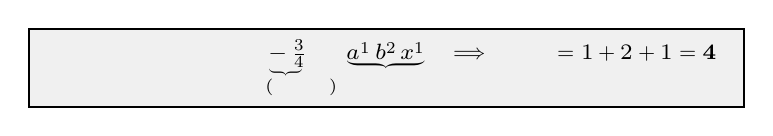
\begin{tikzpicture}
    \node[draw=black, line width=0.8pt, fill=panelgray, inner xsep=10pt, inner ysep=4pt, font=\footnotesize] {គំរូសម្គាល់រចនាសម្ព័ន្ធ៖ \quad $\underbrace{-\frac{3}{4}}_{\text{មេគុណ (រួមទាំងសញ្ញា)}}\;\underbrace{a^{1}\,b^{2}\,x^{1}}_{\text{ផ្នែកអថេរ}} \quad\Longrightarrow\quad \text{ដឺក្រេ} = 1 + 2 + 1 = \mathbf{4}$};
  \end{tikzpicture}
\end{tcolorbox}

\newpage
% ============================================================================
% ទំព័រទី២៖ E4 (លំហាត់គំរូ ទំ.៥២-៥៣) + E5 (ប្រតិបត្តិ + Exit Check) + កិច្ចការផ្ទះ
% ============================================================================

% -------------------- ផ្នែកទី៤៖ E4 ELABORATE --------------------
\secbar{ផ្នែកទី៤ ៖ អនុវត្តលំហាត់គំរូតាមសៀវភៅគោល \enbf{(E4 — Elaborate)}}{\en{10} នាទី (បំពេញតាមគំរូ)}

\textbf{១. លំហាត់គំរូទី១ និងទី២ (សៀវភៅគោល ទំ.៥២)៖}
\begin{itemize}[leftmargin=0.5cm, itemsep=2.5pt, topsep=2pt]
  \item \textbf{គំរូទី១៖} គេមានឯកធា $-\dfrac{3}{4}ab^2x$ $\implies$ \textbf{មេគុណ}គឺ \dotline{2.0cm} \;,\; \textbf{អថេរ}គឺ \dotline{2.5cm} \;,\; \textbf{ផ្នែកអថេរ}គឺ \dotline{2.5cm} ។
  \item \textbf{គំរូទី២៖} ក្នុងចំណោម $5x^2yz^3 \;,\; \dfrac{7}{2}x^2cy^3 \;,\; 5a^2bc^3 \;,\; \dfrac{1}{2}x^2yz^3$ គូ \textbf{ឯកធាដូចគ្នា} គឺ \dotline{2.4cm} និង \dotline{2.4cm} ព្រោះវាមានផ្នែកអថេរ \dotline{2.2cm} ដូចគ្នា (\cnum{3}) ។
\end{itemize}

\vspace{2pt}
\textbf{២. លំហាត់គំរូទី៣ (តារាងដឺក្រេនៃឯកធា ទំ.៥២--៥៣)៖} ចូរបំពេញអថេរ ការបូកនិទស្សន្ត និងដឺក្រេនៃឯកធា៖

\vspace{2pt}
{\renewcommand{\arraystretch}{1.35}
\begin{tabular}{|C{3.5cm}|C{3.5cm}|L{7.2cm}|C{3.4cm}|}
\hline
\cellcolor{headgray}\textbf{ឯកធា} & \cellcolor{headgray}\textbf{អថេរទាំងអស់} & \cellcolor{headgray}\textbf{ការសរសេរនិទស្សន្តលាក់មុខ និងផលបូក} & \cellcolor{headgray}\textbf{ដឺក្រេនៃឯកធា} \\
\hline
$x^2yb^3$ & $x,\; y,\; b$ & $x^2 y^1 b^3 \implies 2 + 1 + 3$ & $\mathbf{6}$ \\
\hline
$\dfrac{3}{4}a^2bc$ & \dotline{2.6cm} & $\dfrac{3}{4}a^2 b^{\Box} c^{\Box} \implies 2 + \dotline{0.9cm} + \dotline{0.9cm}$ & \dotline{1.8cm} \\
\hline
$x^3y^2$ & \dotline{2.6cm} & $x^3 y^2 \implies \dotline{1.2cm} + \dotline{1.2cm}$ & \dotline{1.8cm} \\
\hline
$-3az^2y^3$ & \dotline{2.6cm} & $-3a^{\Box}z^2y^3 \implies \dotline{0.9cm} + 2 + 3$ & \dotline{1.8cm} \\
\hline
\end{tabular}}

\vspace{3pt}
$\bullet$ \textbf{សំណួរឆ្លុះបញ្ចាំង (\en{Looking Back})៖} ហេតុអ្វីកន្សោម $\sqrt{5}ax^2$ ជាឯកធា តែ $5\sqrt{x}$ មិនមែនជាឯកធា?\\
ចម្លើយ៖ ព្រោះក្នុង $\sqrt{5}ax^2$ សញ្ញារ៉ាឌីកាល់នៅលើ \dotline{3.5cm} ចំណែកក្នុង $5\sqrt{x}$ សញ្ញារ៉ាឌីកាល់នៅលើ \dotline{3.5cm} ។

% -------------------- ផ្នែកទី៥៖ E5 EVALUATE --------------------
\secbar{ផ្នែកទី៥ ៖ ហ្វឹកហាត់ «ប្រតិបត្តិ» និងតេស្តរហ័ស \enbf{(E5 — Evaluate)}}{\en{10} នាទី (ធ្វើដោយខ្លួនឯង រួចប្ដូរផ្ទៀង)}

\textbf{១. លំហាត់ប្រតិបត្តិ (សៀវភៅគោល ទំ.៥២)៖}
\begin{enumerate}[label=\alph*), leftmargin=0.55cm, itemsep=2.5pt, topsep=2pt]
  \item ចូរបញ្ជាក់មេគុណ និងអថេរនៃឯកធា $2\sqrt{3}yt^2$ ៖ មេគុណ $= \dotline{2.3cm}$ \;,\; អថេរ $= \dotline{2.5cm}$ \;,\; ដឺក្រេ $= \dotline{1.6cm}$ ។
  \item ចូរជ្រើសរើស \textbf{ឯកធាដូចគ្នា} ក្នុងចំណោម៖ $\dfrac{1}{2}xy \;,\; -2x^2y \;,\; ay \;,\; 3ax \;,\; 2xy^2 \;,\; xy$ ។\\
  ចម្លើយ៖ គូឯកធាដូចគ្នាគឺ \dotline{2.8cm} និង \dotline{2.8cm} (ព្រោះមានផ្នែកអថេរ \dotline{2.2cm} ដូចគ្នា) ។
\end{enumerate}

\vspace{2pt}
\textbf{២. លំហាត់ប្រតិបត្តិ (សៀវភៅគោល ទំ.៥៣)៖} ចូរកំណត់អថេរ និងរកដឺក្រេនៃឯកធានីមួយៗខាងក្រោម៖

\vspace{2pt}
{\renewcommand{\arraystretch}{1.35}
\begin{tabular}{|L{2.8cm}|C{2.8cm}|L{3.1cm}||L{2.8cm}|C{2.8cm}|L{3.1cm}|}
\hline
\cellcolor{headgray}\textbf{ឯកធា} & \cellcolor{headgray}\textbf{អថេរ} & \cellcolor{headgray}\textbf{ដឺក្រេ} &
\cellcolor{headgray}\textbf{ឯកធា} & \cellcolor{headgray}\textbf{អថេរ} & \cellcolor{headgray}\textbf{ដឺក្រេ} \\
\hline
ក. $\dfrac{1}{2}xyz$ & \dotline{2.1cm} & \dotline{2.3cm} & ឃ. $21ab^4c$ & \dotline{2.1cm} & \dotline{2.3cm} \\
\hline
ខ. $8x^3yz^2$ & \dotline{2.1cm} & \dotline{2.3cm} & ង. $3x^2y^3z^4$ & \dotline{2.1cm} & \dotline{2.3cm} \\
\hline
គ. $14$ & \dotline{2.1cm} & \dotline{2.3cm} & ច. $axyz$ & \dotline{2.1cm} & \dotline{2.3cm} \\
\hline
\end{tabular}}

\vspace{4pt}
\begin{tcolorbox}[enhanced, sharp corners, colback=panelgray, colframe=black, boxrule=0.85pt, top=3pt, bottom=3pt, left=6pt, right=6pt]
  \textbf{៣. បិទបេសកកម្ម \en{E1} និងតេស្តរហ័ស (\en{Exit Check — 60} វិនាទី)៖}\\[2pt]
  $\bullet$ \textbf{ចម្លើយបេសកកម្ម \en{E1}៖} ឯកធា $x^2yb^3 = x^2y^1b^3$ មានដឺក្រេស្មើ $\dotline{1.2cm} + \dotline{1.2cm} + \dotline{1.2cm} = \dotline{1.5cm}$ ។\\[2pt]
  $\bullet$ \textbf{សំណួរតេស្តរហ័ស៖} តើឯកធា $-\dfrac{5}{7}m^3np^4$ មានមេគុណ និងដឺក្រេស្មើប៉ុន្មាន? (គូសរង្វង់ជម្រើសត្រឹមត្រូវតែមួយ)៖\\[2pt]
  \hspace*{0.3cm}\enbf{A.}\; មេគុណ $\dfrac{5}{7}$, ដឺក្រេ $7$ \qquad
  \enbf{B.}\; មេគុណ $-\dfrac{5}{7}$, ដឺក្រេ $7$ \qquad
  \enbf{C.}\; មេគុណ $-\dfrac{5}{7}$, ដឺក្រេ $8$ \qquad
  \enbf{D.}\; មេគុណ $-\dfrac{5}{7}$, ដឺក្រេ $12$
\end{tcolorbox}

% -------------------- ផ្នែកទី៦៖ កិច្ចការផ្ទះ --------------------
\secbar{ផ្នែកទី៦ ៖ ប័ណ្ណកិច្ចការផ្ទះ \enbf{(Homework)} និងការអានជាមុន}{សៀវភៅសិក្សាគោល ទំព័រ ៧២}

\begin{tcolorbox}[enhanced, sharp corners, colback=white, colframe=black, boxrule=0.8pt, borderline={0.6pt}{2pt}{dashed}, top=3pt, bottom=3pt, left=6pt, right=6pt]
  \textbf{១. លំហាត់ទី១ (ទំ.៧២)៖} តើកន្សោមខាងក្រោមមួយណាជាឯកធា? ចំពោះកន្សោមដែលជាឯកធា ចូរបញ្ជាក់មេគុណ និងដឺក្រេរបស់វា៖
  \[ \frac{x^3}{3} \quad,\quad \sqrt{5}ax^2 \quad,\quad \frac{7xy^2}{3} \quad,\quad x + 2y \quad,\quad \frac{a}{x^2} \quad,\quad x(x+y) \]
  \textbf{២. លំហាត់បង្កើតគំរូ៖} ចូរសរសេរឯកធាពីរដែលជា \textbf{ឯកធាដូចគ្នា} មានអថេរ $x, y$ និងមានដឺក្រេស្មើ $5$ (ធ្វើក្នុងសៀវភៅកិច្ចការផ្ទះ) ។\\[1.5pt]
  $\bullet$ \textbf{អានជាមុន៖} ចំណុច \textbf{១.៤--១.៦ ប្រមាណវិធីបូក ដក គុណ និងចែកឯកធា} (សៀវភៅគោល ទំព័រ ៥៣--៥៦) ។
\end{tcolorbox}

\end{document}
